\begin{appendix}
\chapter{Listado de características}\label{AnexoA}
A continuación se enumeran todas las características numéricas que son utilizadas en este trabajo para describir una curva de luz. El primer subgrupo fue generado utilizando la herramienta Feets \cite{cabral2018fats}, mientras que el segundo subgrupo son características de color introducidas en \cite{jbc}

\section{Características extraídas utilizando Feets}
Las descripciones de este listado están basadas en la documentación de Feets \url{https://feets.readthedocs.io}:

\begin{itemize}
\item \textbf{Amplitude}: La mitad de la diferencia entre la mediana del 5\% de los valores mayores y la mediana del 5\% de los valores más pequeños de las magnitudes en la banda $K_S$.

\item \textbf{Autocolor\_length}: (Auto-Correlation Length) Correlación cruzada de la señal con si misma. Es útil para encontrar patrones, como señales periódicas, ocultas por ruido.

\item \textbf{Beyond1Std}: Porcentaje de puntos más allá de una desviación estándar de la media ponderada.

\item \textbf{Con}: (Consecutive points) Cantidad de tres puntos consecutivos mayores o menores que $2\sigma$ (normalizado por  $N-200$). 

\item \textbf{Eta\_e}: Verifica la dependencia de  observaciones con respecto a las anteriores.

\item \textbf{FluxPercentileRatioMid}: (Proporción del flujo de percentiles centrales) Caracteriza las distribuciones de magnitud ordenadas en base a percentiles de sus flujos\footnote{Flujo o luminosidad, es la cantidad de energía que brinda una estrella en una unidad de tiempo}. Se calcularon las siguientes cinco features, donde $F_{i,j}$ es la diferencia entre el percentil de flujo $j$ y el percentil de flujo $i$:
	\begin{itemize}
	\item FluxPercentileRatioMid20 = $F_{40,60} / F_{5,95}$
	\item FluxPercentileRatioMid35 = $F_{32.5,67.5} / F_{5,95}$
	\item FluxPercentileRatioMid50 = $F_{25,75} / F_{5,95}$
	\item FluxPercentileRatioMid65 = $F_{17.5,82.5} / F_{5,95}$
	\item FluxPercentileRatioMid80 = $F_{10,90} / F_{5,95}$
	\end{itemize}

\item \textbf{Componentes de Fourier}: Las primeras tres componentes de Fourier para los primeros tres períodos candidatos. \textit{Freqk\_harmonics\_amplitude\_i} y \textit{Freqk\_harmonics\_rel\_phase\_j} representan la i-ésima amplitud y la j-ésima fase de la señal para el k-ésimo período candidato. (Un total de 18 features)

\item \textbf{Gskew}: Medida de distorsión basada en la mediana de magnitudes.

\item \textbf{LinearTrend}: (Tendencia linear) Es la pendiente del ajuste lineal de los datos.

\item \textbf{MaxSlope}: Pendiente máxima absoluta entre dos observaciones consecutivas.

\item \textbf{Mean}: Media de magnitudes.
\item \textbf{MedianAbsDev}: (Mediana de las desviaciones absolutas) La mediana de la diferencia de cada magnitud observada con la mediana de la serie.
\item \textbf{MedianBRP}: (Median Buffer Range Percentage) Proporción de las magnitudes entre la décima parte del rango total alrededor de la mediana.
\item \textbf{PairSlopeTrend}: Tendencia de pendiente de a pares.
\item \textbf{PercentAmplitude}: (Porcentaje de Amplitud) Máximo porcentaje de diferencia entre la máxima o la mínima magnitud y su mediana.
\item \textbf{PercentDifferenceFluxPercentile}: $F_{5,95}$ convertido a magnitud.
\item \textbf{PeriodLS}: Período extraído usando el método de Lomb-Scargle.
\item \textbf{Period\_fit}: (Period Fitness) Medida de la confiabilidad de PeriodLS.
\item \textbf{Psi\_CS}: Índice $R_CS$ aplicado a la curva en fase, utilizando el período extraído con el método de Lomb-Scargle.
\item \textbf{Psi\_eta}: Índice $\eta^e$ calculado con la curva de luz puesta en fase con el período extraído con el método de Lomb-Scargle.
\item \textbf{Q31}: Diferencia entre el tercer cuartil y el primer cuartil de magnitudes.
\item \textbf{Rcs}: (Range Cumulative Sum) Rango obtenido luego de calcular la suma acumulada de mediciones.
\item \textbf{Skew}: La asimetría de las magnitudes.
\item \textbf{SmallKurtosis}: Kurtosis pequeña de las magnitudes.
\item \textbf{Std}: La desviación estándar de las magnitudes.
\end{itemize}

\section{Características de color}

A continuación se encuentra el listado de features relativas al color de una estrella que se utilizaron en este trabajo.

\begin{itemize}
\item \textbf{c89\_c3}: C3 Pseudo-color usando la Ley de Extinción de Cardelli-89.
\item \textbf{c89\_ab\_color}: Diferencia de magnitud en la primera época entre la banda a y la banda b, usando la Ley de Extinción de Cardelli-89. a y b pueden ser las bandas H, J y Ks.
\item \textbf{c89\_m2} y \textbf{c89\_m4}: Pseudo-magnitudes m2 y m4  usando la Ley de Extinción de Cardelli-89.
\item \textbf{n09\_c3}: C3 Pseudo-color usando la Ley de Extinción de Nishiyama-09.
\item \textbf{n09\_ab\_color}: Diferencia de magnitud en la primera época entre la banda a y la banda b, usando la Ley de Extinción de Nishiyama-09. a y b pueden ser las bandas H, J y Ks.
\item \textbf{n09\_m2} y \textbf{n09\_m4}: Pseudo-magnitudes m2 y m4 usando la Ley de Extinción de Nishiyama-09.
\item \textbf{ppmb} (Pseudo-Phase Multi-Band): Este índice setea el primer instante en fase con respecto al tiempo promedio en todas las bandas, usando el período calculado por Feets: \\

\begin{center}
$ ppmb = frac (\frac{|mean(HJD_H, HJD_J, HJD_{K_s}) - T_0|}{P}) $

\end{center}

Donde $HJD_H$, $HJD_J$ y $HJD_K$ son el tiempo de las observaciones en las bandas $H$, $J$  y $K_S$; y $T_0$ es el tiempo de observación de la máxima magnitud en la banda $K_S$. P es el período extraído. $frac$ retorna sólo la parte decimal del número.
\end{itemize}


Para más información acerca de la Ley de Extinción de Cardelli-89, consultar \cite{cardelli}. Para más información acerca de la Ley de Extinción de Nishiyama-09, consultar \cite{Nishiyama}. Para más información acerca de pseudo colores, consultar \cite{vvv}

\section{Índice de atributos}
\label{indice_atributos}
A continuación se enumeran todos los atributos nuevamente, así como un número identificador para cada uno. Estos identificadores serán utilizados para referirse al nombre de cada atributo en distintas secciones del trabajo. 

\begin{multicols}{2}
\begin{enumerate}[noitemsep]
\setcounter{enumi}{-1}
\item Amplitude
\item Autocor\_length
\item Beyond1Std
\item Con
\item Eta\_e
\item FluxPercentileRatioMid20
\item FluxPercentileRatioMid35
\item FluxPercentileRatioMid50
\item FluxPercentileRatioMid65
\item FluxPercentileRatioMid80
\item Freq1\_harmonics\_amplitude\_0
\item Freq1\_harmonics\_amplitude\_1
\item Freq1\_harmonics\_amplitude\_2
\item Freq1\_harmonics\_amplitude\_3
\item Freq1\_harmonics\_rel\_phase\_1
\item Freq1\_harmonics\_rel\_phase\_2
\item Freq1\_harmonics\_rel\_phase\_3
\item Freq2\_harmonics\_amplitude\_0
\item Freq2\_harmonics\_amplitude\_1
\item Freq2\_harmonics\_amplitude\_2
\item Freq2\_harmonics\_amplitude\_3
\item Freq2\_harmonics\_rel\_phase\_1
\item Freq2\_harmonics\_rel\_phase\_2
\item Freq2\_harmonics\_rel\_phase\_3
\item Freq3\_harmonics\_amplitude\_0
\item Freq3\_harmonics\_amplitude\_1
\item Freq3\_harmonics\_amplitude\_2
\item Freq3\_harmonics\_amplitude\_3
\item Freq3\_harmonics\_rel\_phase\_1
\item Freq3\_harmonics\_rel\_phase\_2
\item Freq3\_harmonics\_rel\_phase\_3
\item Gskew
\item LinearTrend
\item MaxSlope
\item Mean
\item MedianAbsDev
\item MedianBRP
\item PairSlopeTrend
\item PercentAmplitude
\item PercentDifferenceFluxPercentile
\item PeriodLS
\item Period\_fit
\item Psi\_CS
\item Psi\_eta
\item Q31
\item Rcs
\item Skew
\item SmallKurtosis
\item Std
\item c89\_c3
\item c89\_hk\_color
\item c89\_jh\_color
\item c89\_jk\_color
\item c89\_m2
\item c89\_m4
\item n09\_c3
\item n09\_hk\_color
\item n09\_jh\_color
\item n09\_jk\_color
\item n09\_m2
\item n09\_m4
\item ppmb
\end{enumerate}
\end{multicols}

\chapter{Anexo B}\label{anexoB}

\section{Tests estadísticos - pvalues}
\label{anexo_b_pvalues}
 En esta sección se muestran los p-values de los tests $\chi^2$ y ANOVA, complementando la figura \ref{fig:pvalues_b278}.
 
\begin{figure}[h!]
\centering
  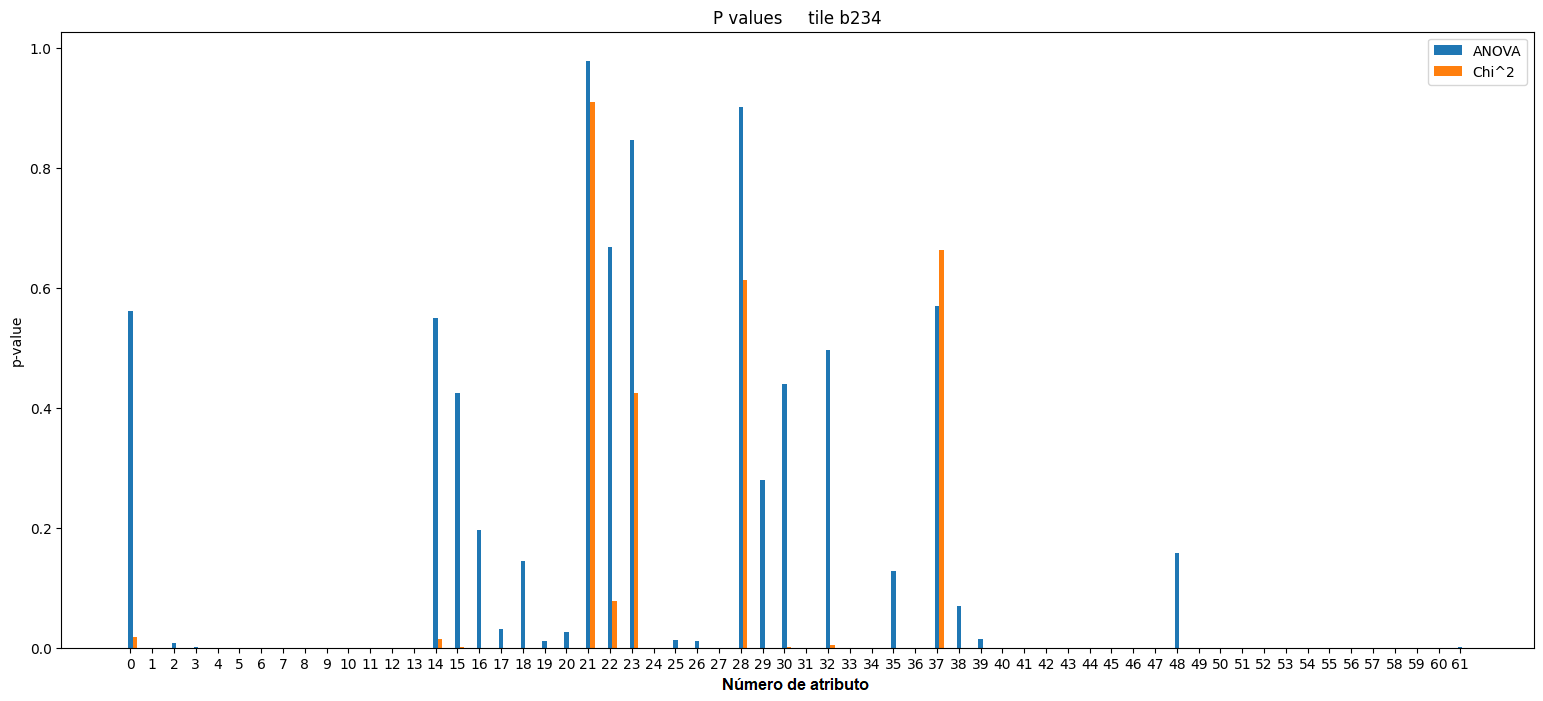
\includegraphics[width=0.49\textwidth]{Kap6/test=b234_variable_importance_pvalues.png}  
  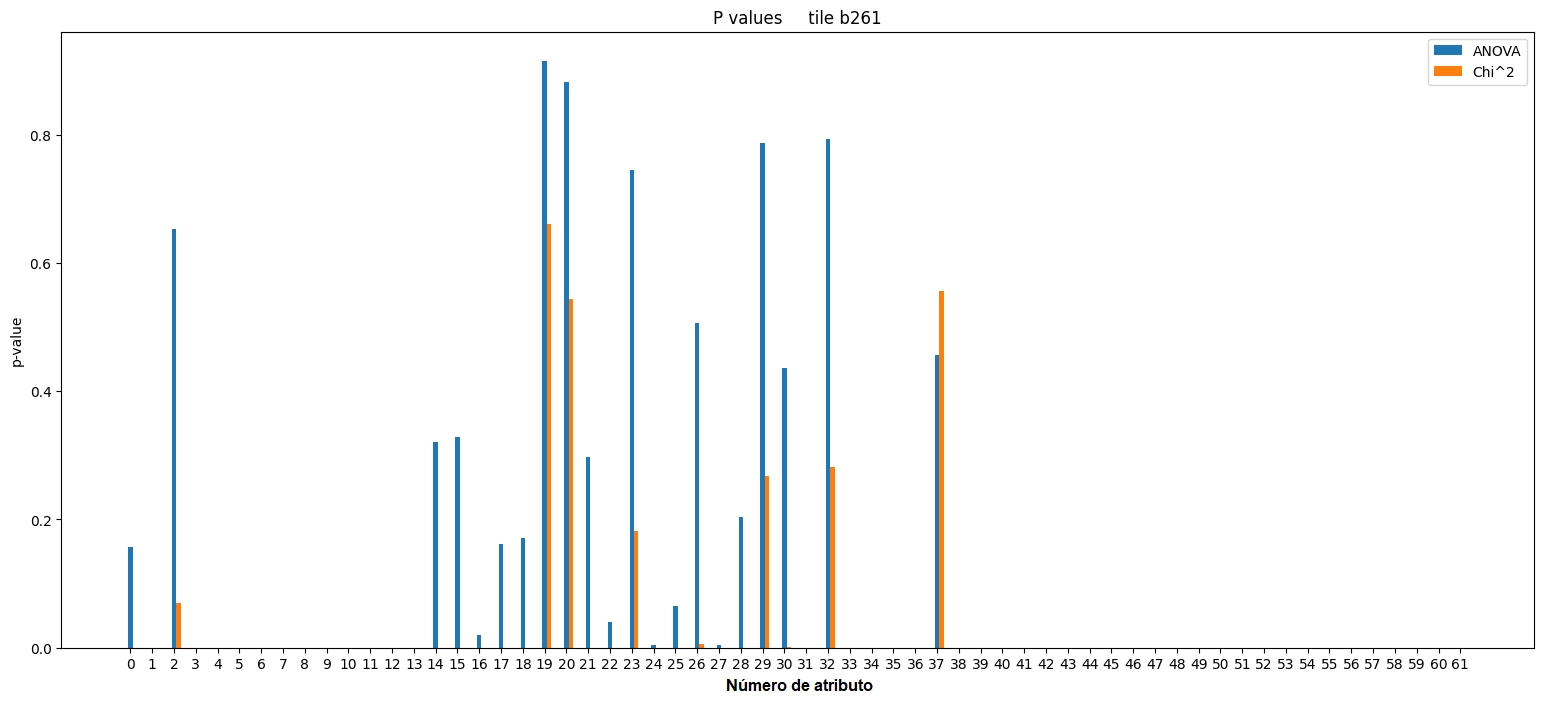
\includegraphics[width=0.49\textwidth]{Kap6/test=b261_variable_importance_pvalues.png} \\
  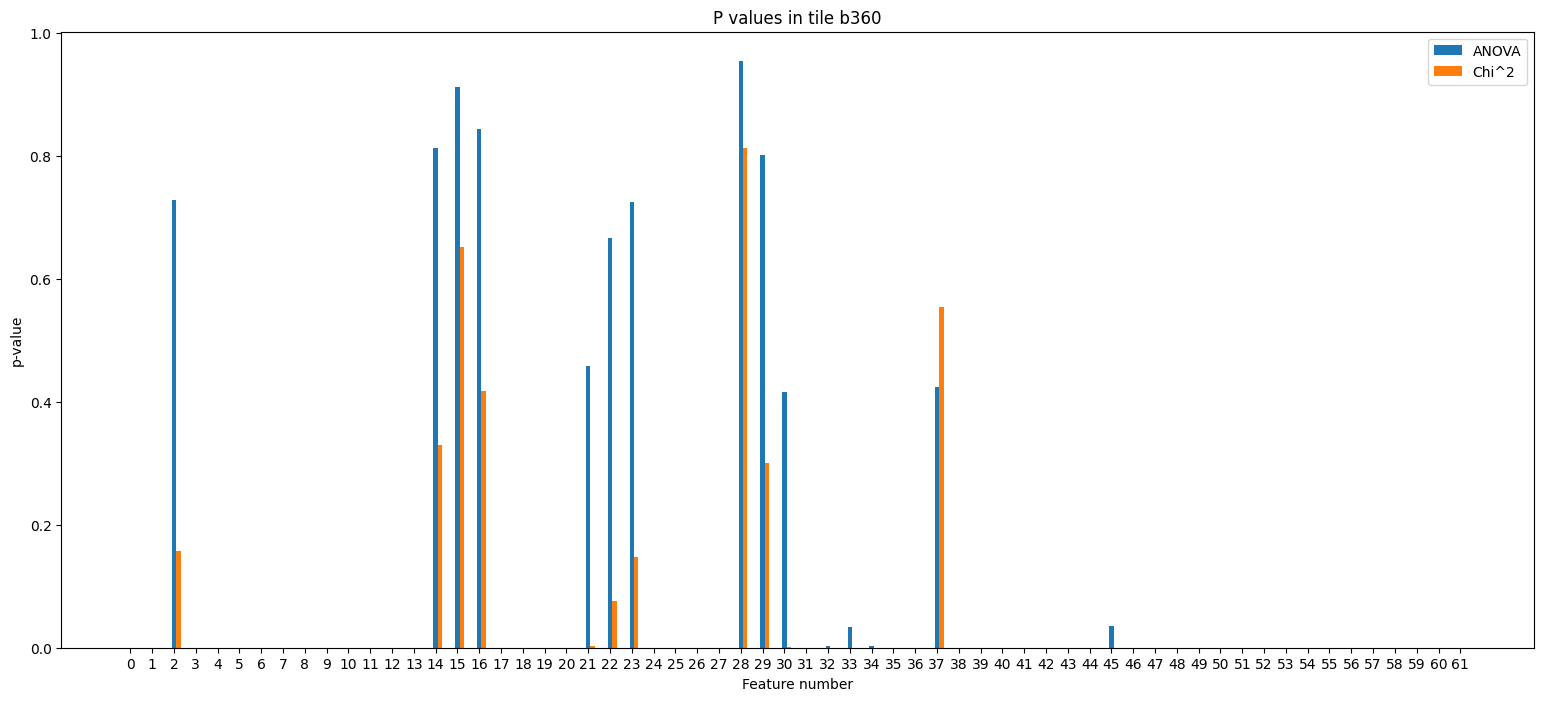
\includegraphics[width=0.49\textwidth]{Kap6/test=b360_variable_importance_pvalues.png} 
\end{figure}

\section{Tests estadísticos - métricas}
\label{anexo_b_scores}
 En esta sección se muestran los puntajes de los tests $\chi^2$ y ANOVA, así como la información mutua, complementando la figura \ref{fig:scores_b278}.
 
\begin{figure}[h!]
\centering
  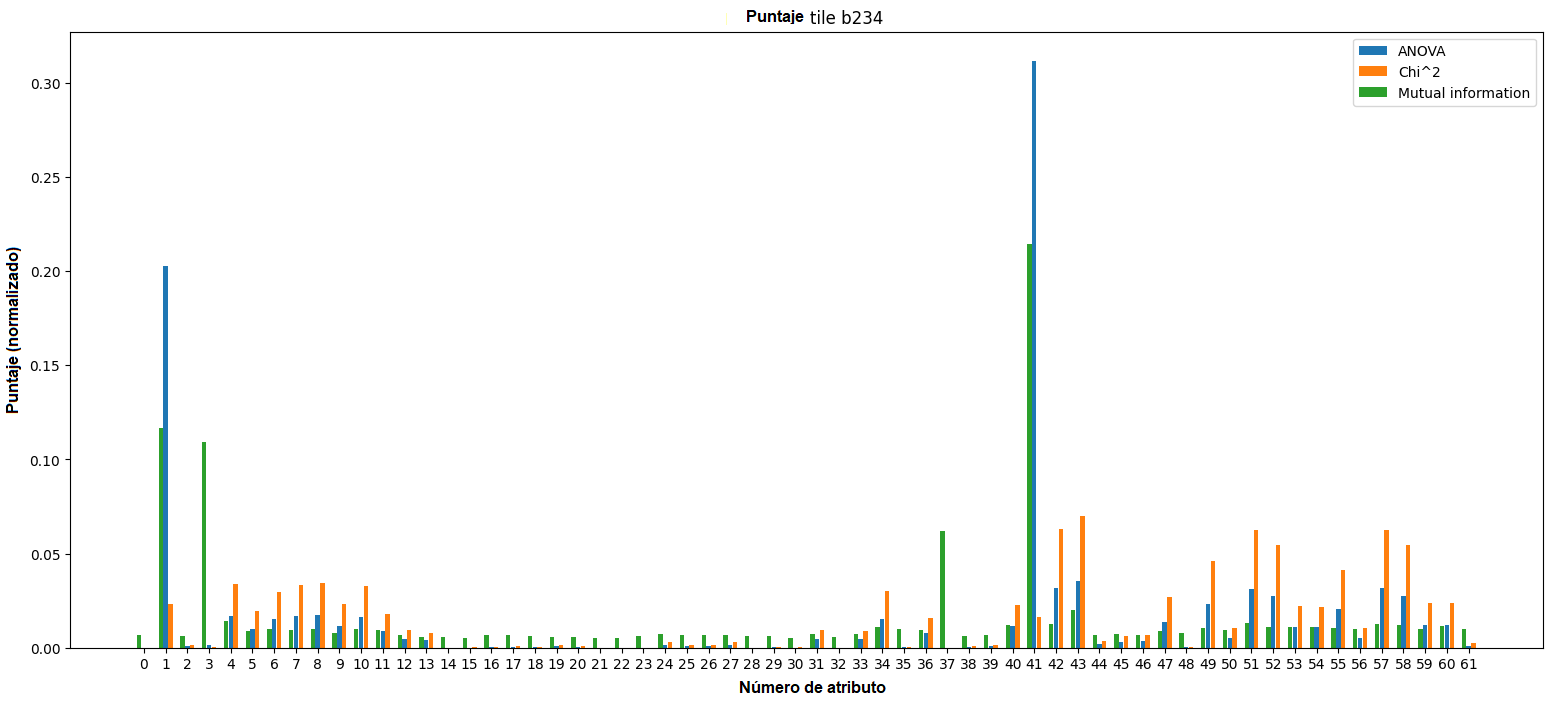
\includegraphics[width=0.49\textwidth]{Kap6/test=b234_variable_importance_scores.png} 
  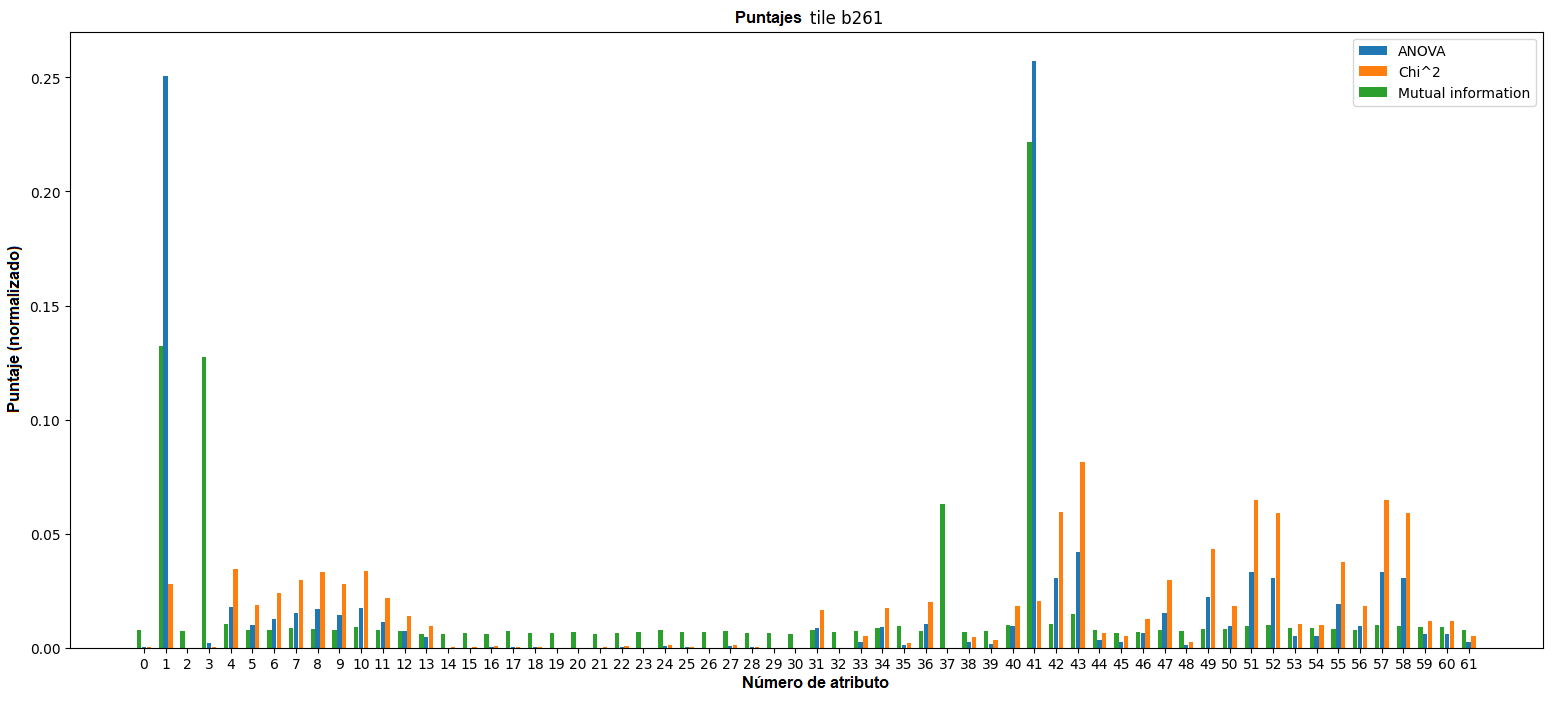
\includegraphics[width=0.49\textwidth]{Kap6/test=b261_variable_importance_scores.png} 
  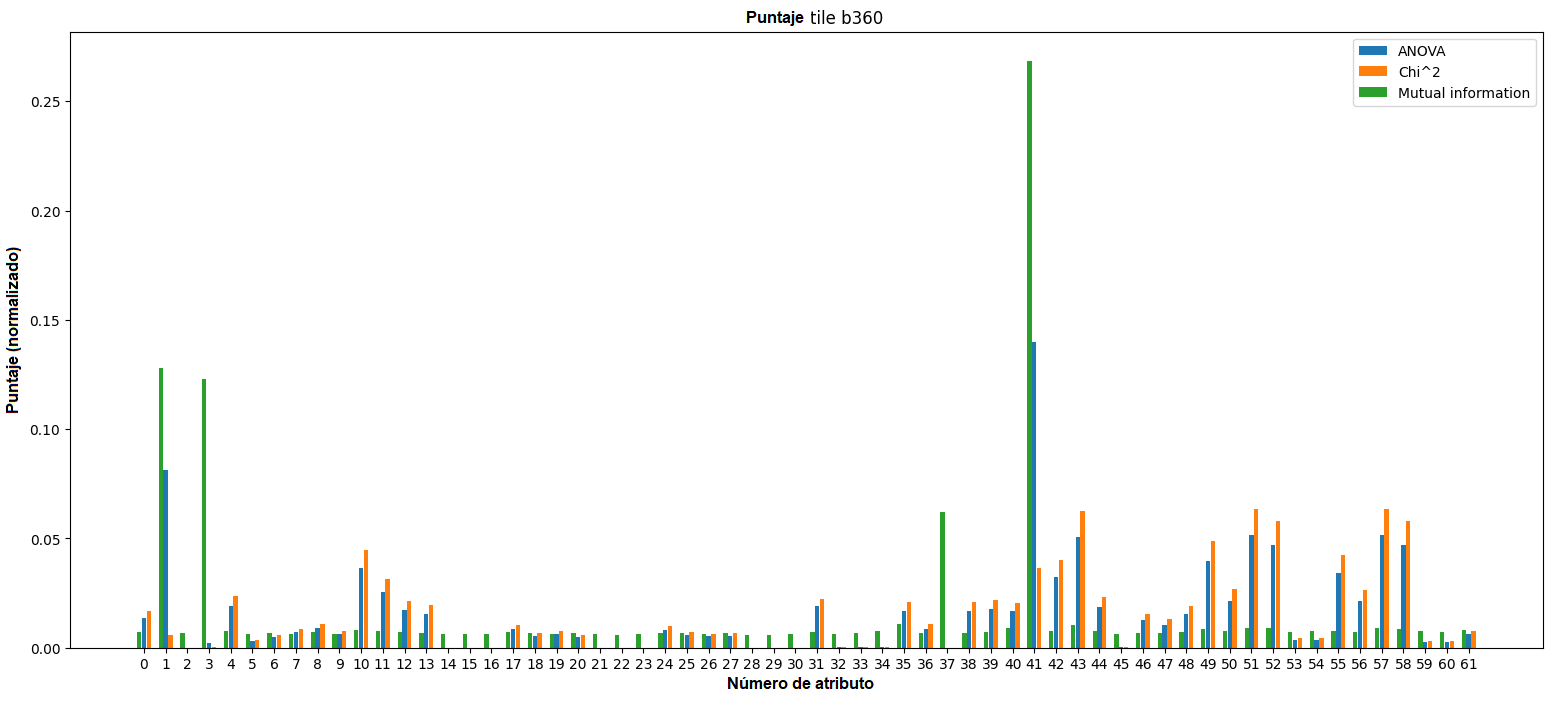
\includegraphics[width=0.49\textwidth]{Kap6/test=b360_variable_importance_scores.png} 
\end{figure}

\newpage

\section{Tests estadísticos - rankings}
\label{anexo_b_rankings}
 En esta sección se muestran los rankings de variables generados por los tests $\chi^2$ y ANOVA, así como por información mutua, complementando la figura \ref{fig:ranking_b278}.
 
\begin{figure}[h!]
\centering
  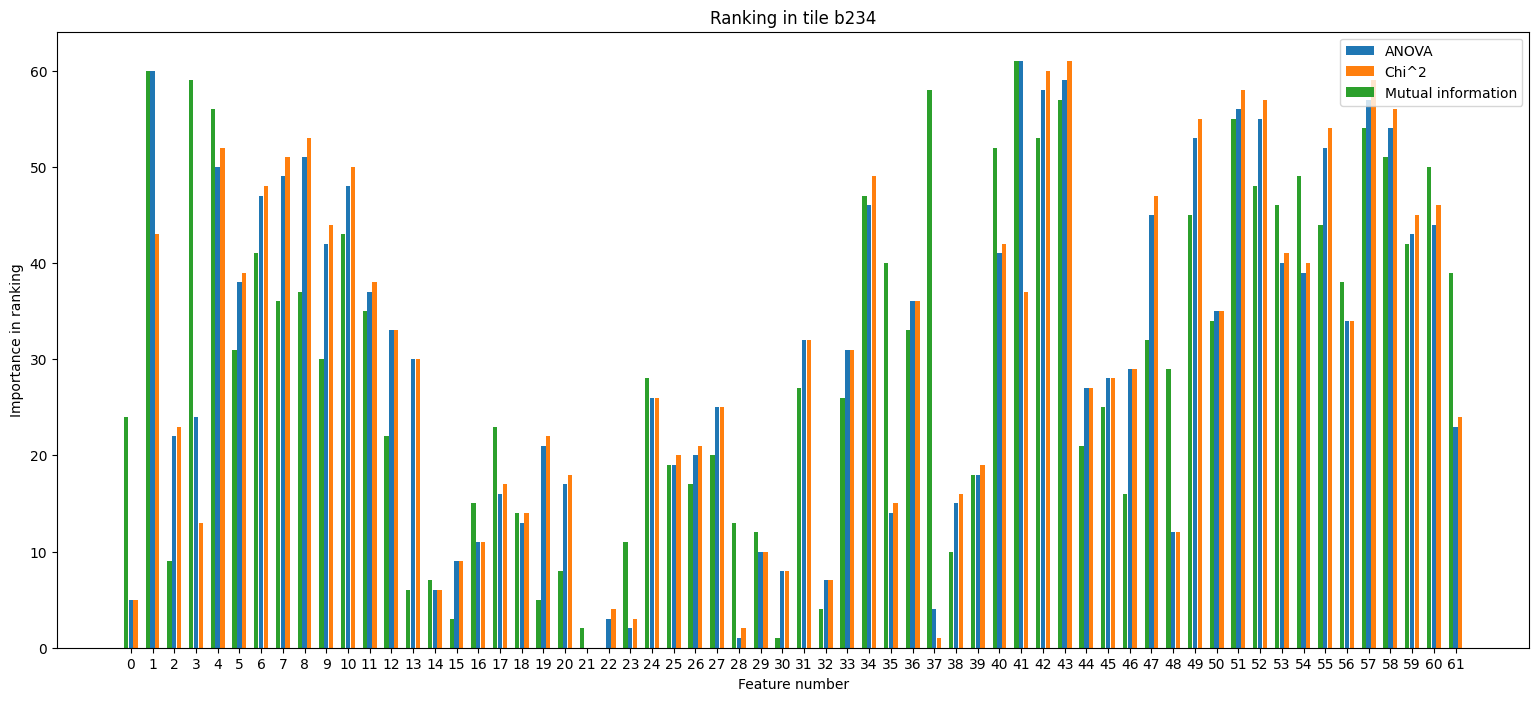
\includegraphics[width=0.49\textwidth]{Kap6/test=b234_variable_importance_ranking.png} 
  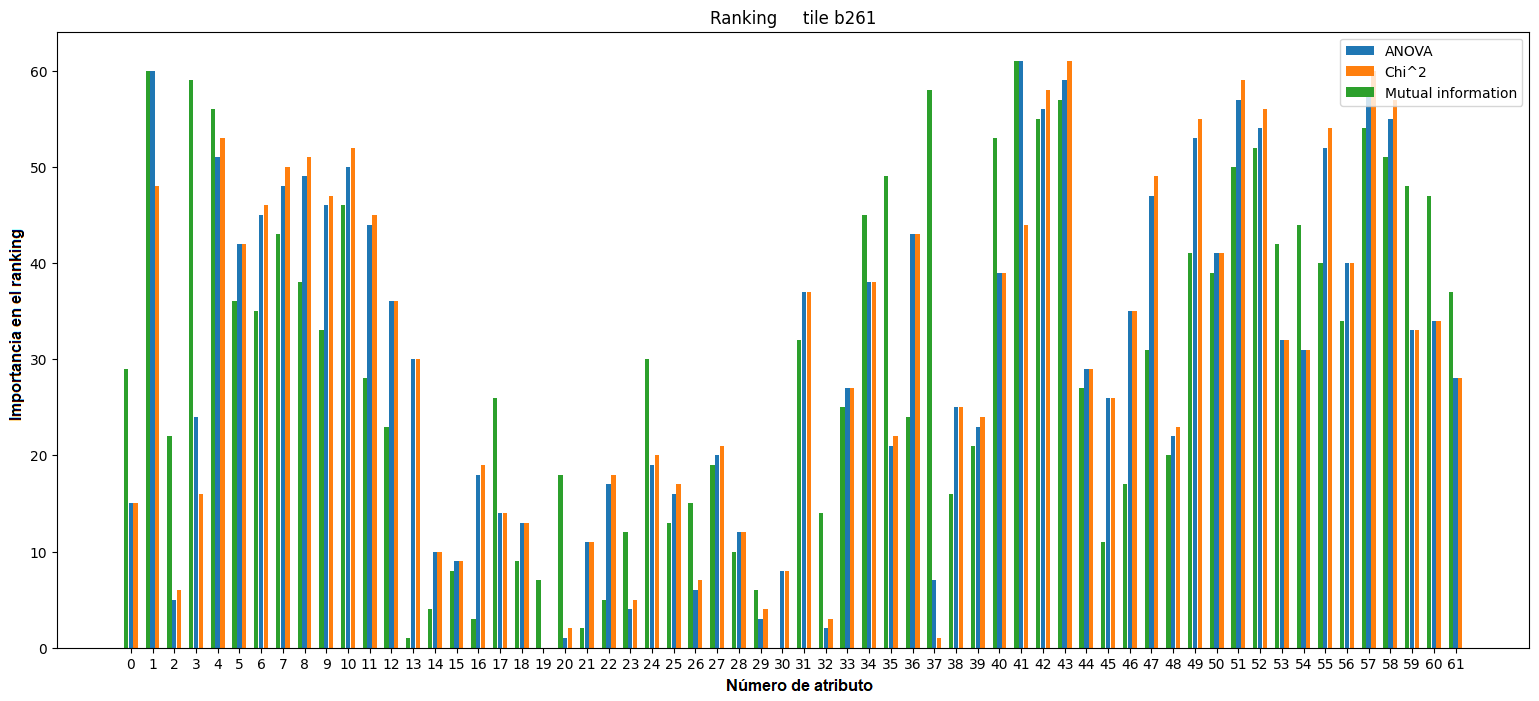
\includegraphics[width=0.49\textwidth]{Kap6/test=b261_variable_importance_ranking.png}  \\
  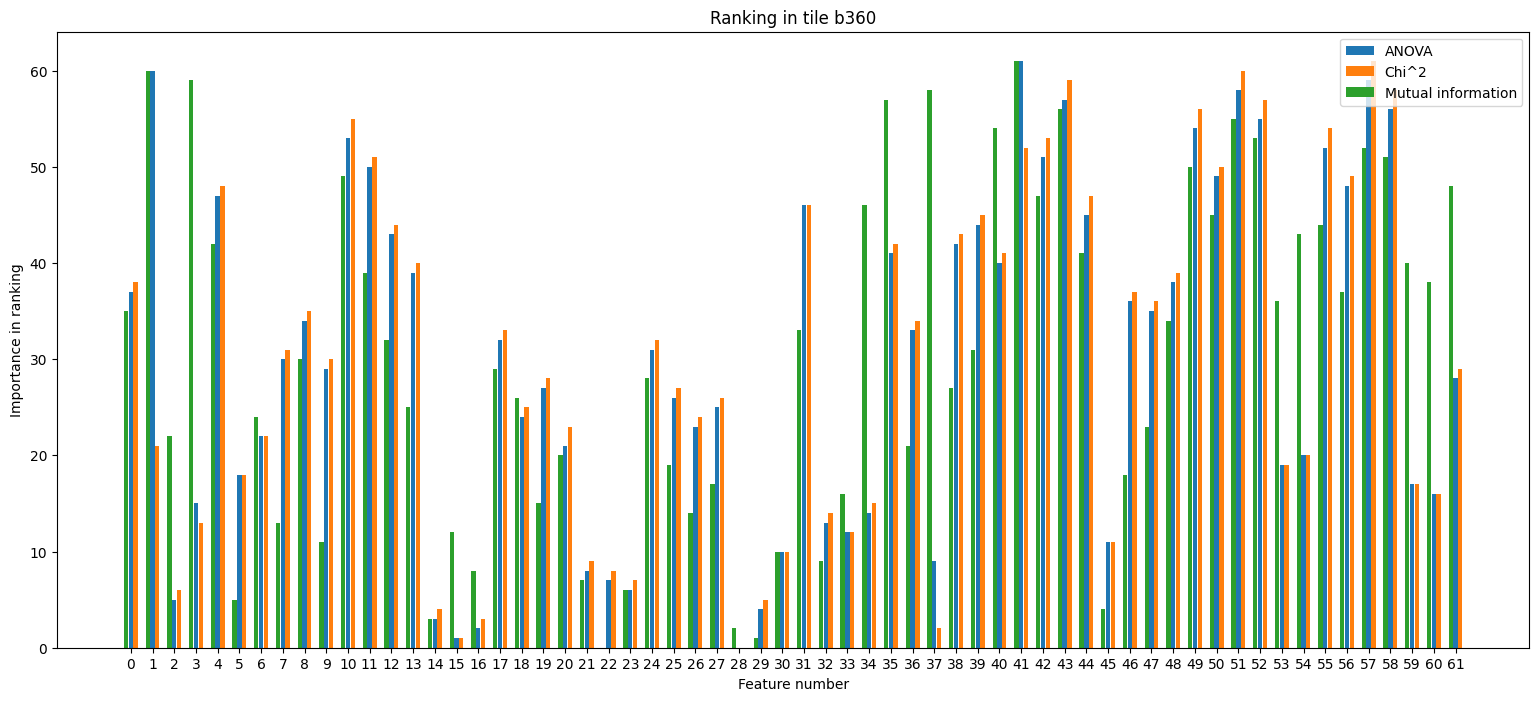
\includegraphics[width=0.49\textwidth]{Kap6/test=b360_variable_importance_ranking.png} 
\end{figure}

\section{Importancia de atributos basado en clasificadores}
\label{anexo_ml_scores}
 En esta sección se muestra la importancia asignada por SVM-Lineal y RF en distintos tiles, y complementando la figura \ref{fig:ml_importance_b278}.
 
\begin{figure}[h!]
\centering
  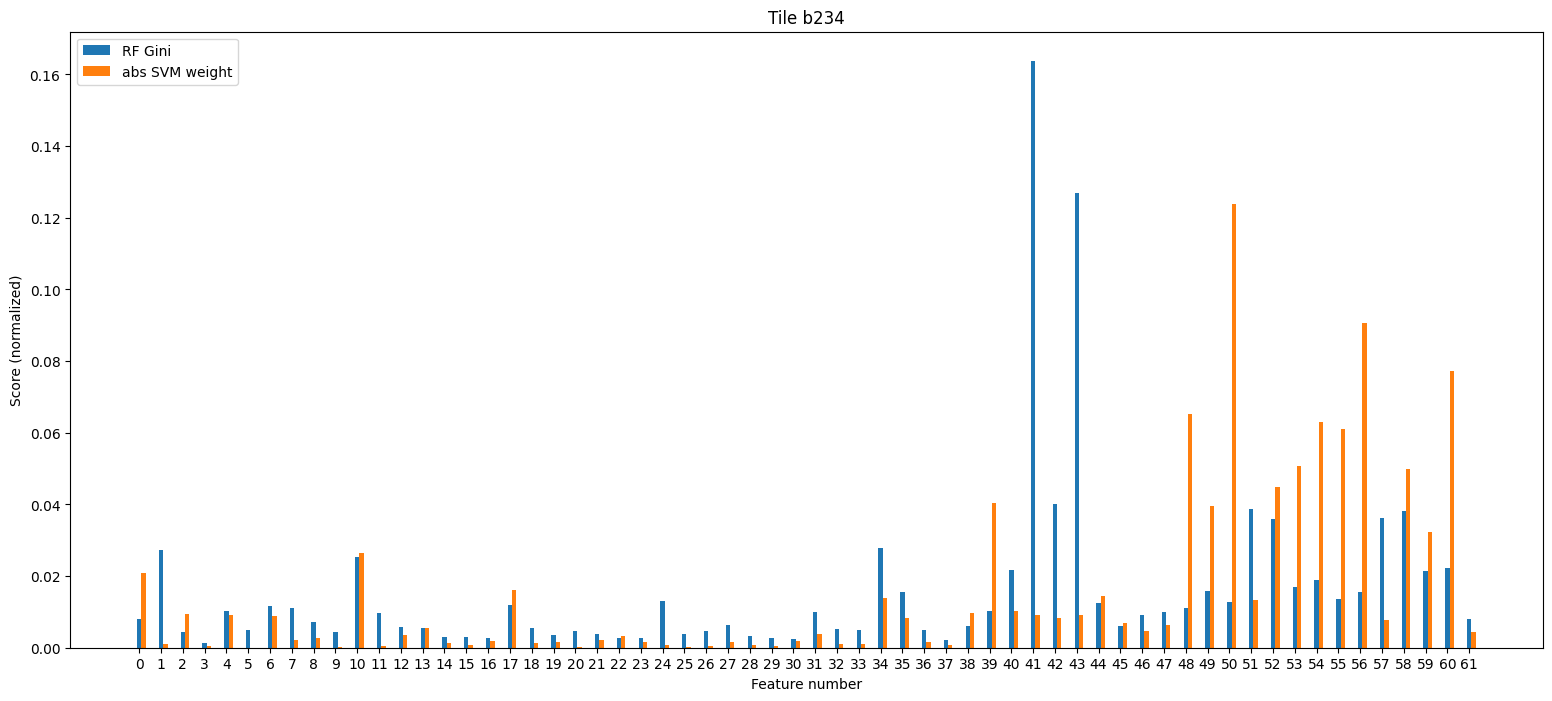
\includegraphics[width=0.49\textwidth]{Kap6/test=b234_ML_variable_importance_scores.png} 
  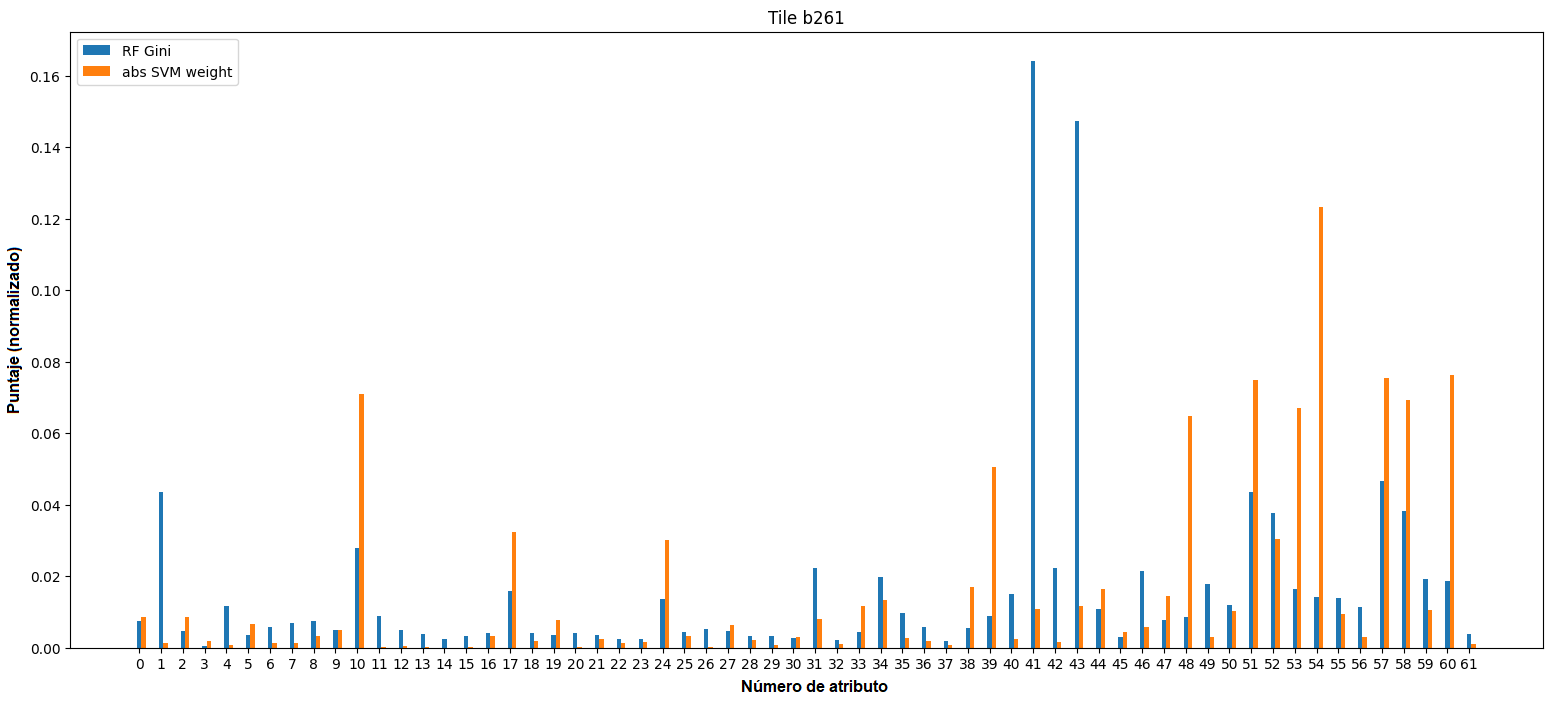
\includegraphics[width=0.49\textwidth]{Kap6/test=b261_ML_variable_importance_scores.png} \\
  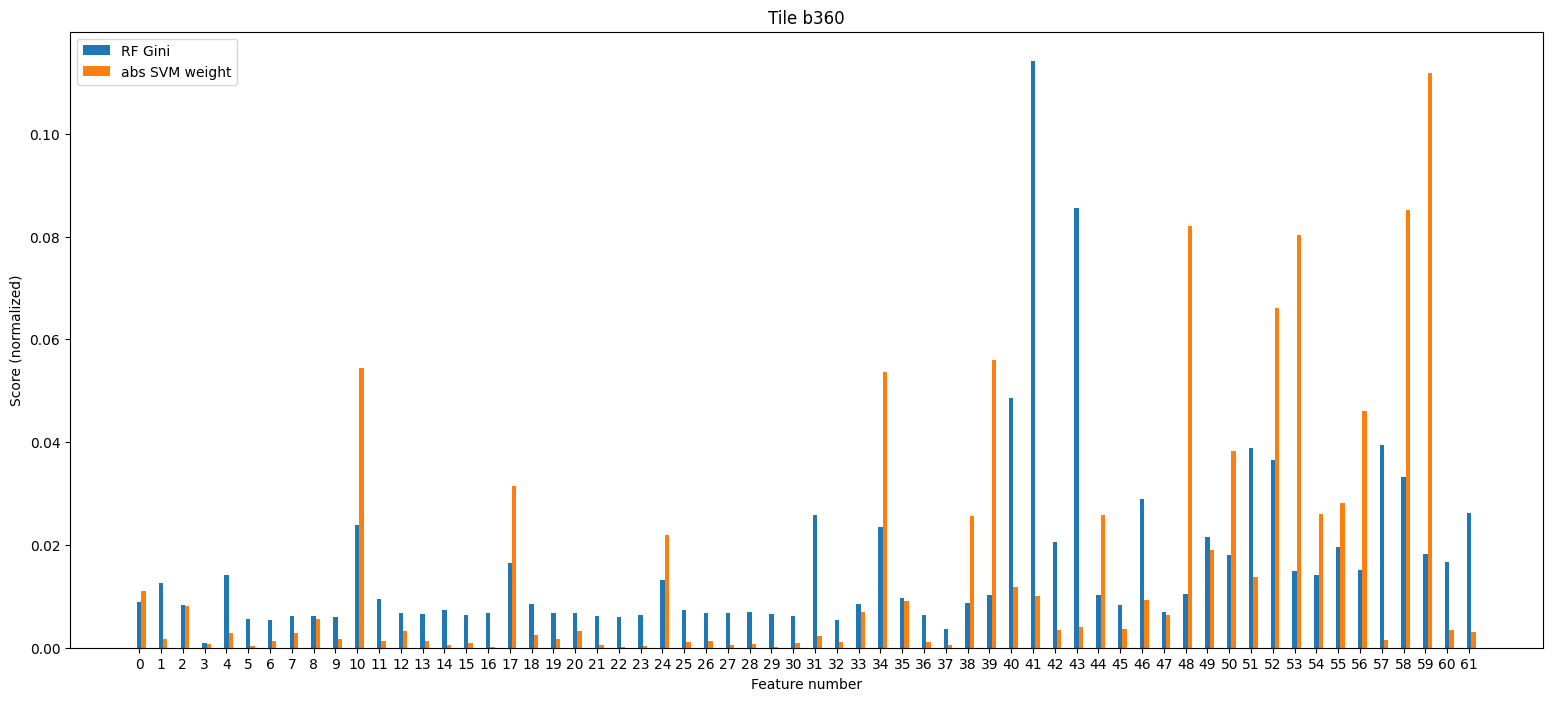
\includegraphics[width=0.49\textwidth]{Kap6/test=b360_ML_variable_importance_scores.png} 
\end{figure}

\section{Matrices de correlación entre atributos}
\label{anexo_matrices_correlacion}
En esta sección se muestra el coeficiente de correlación para cada par de atributos en los tiles b234, b261 y b360.

\begin{figure}[h!]
\centering
  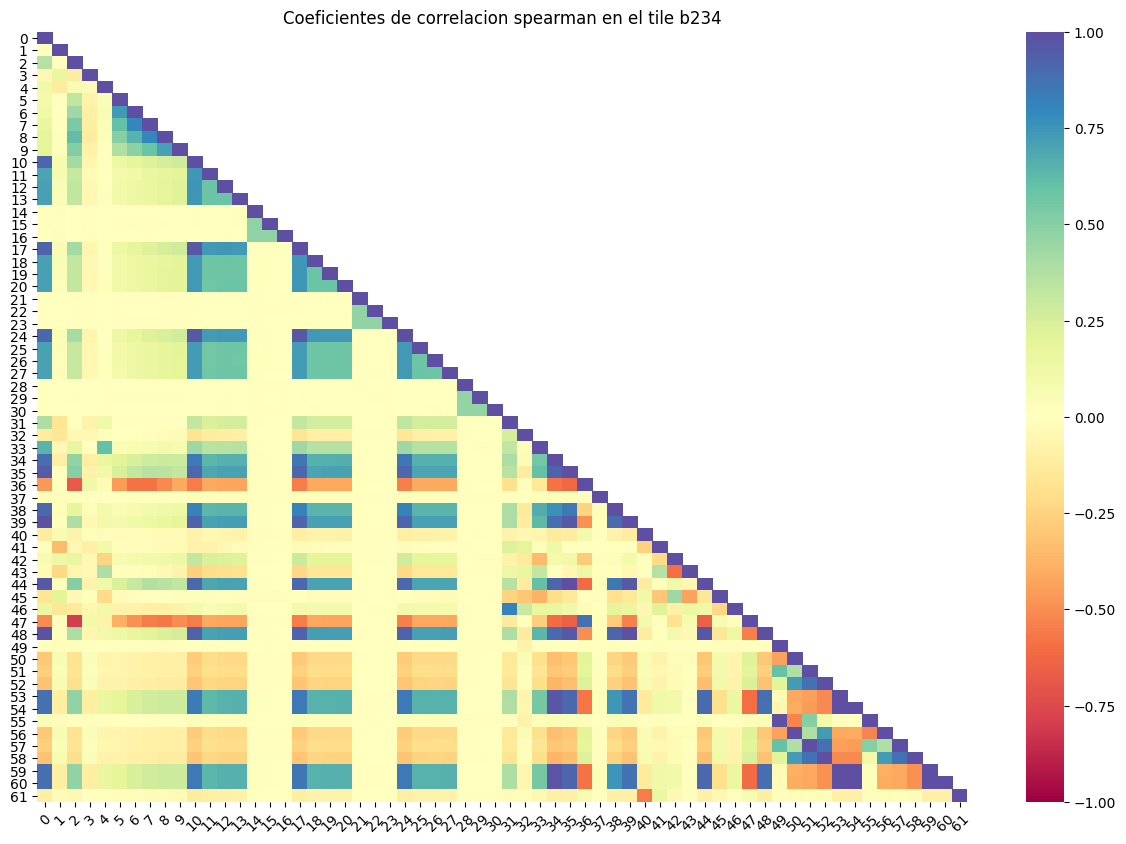
\includegraphics[width=0.49\textwidth]{Kap6/spearman_b234_MATRIX.png} 
  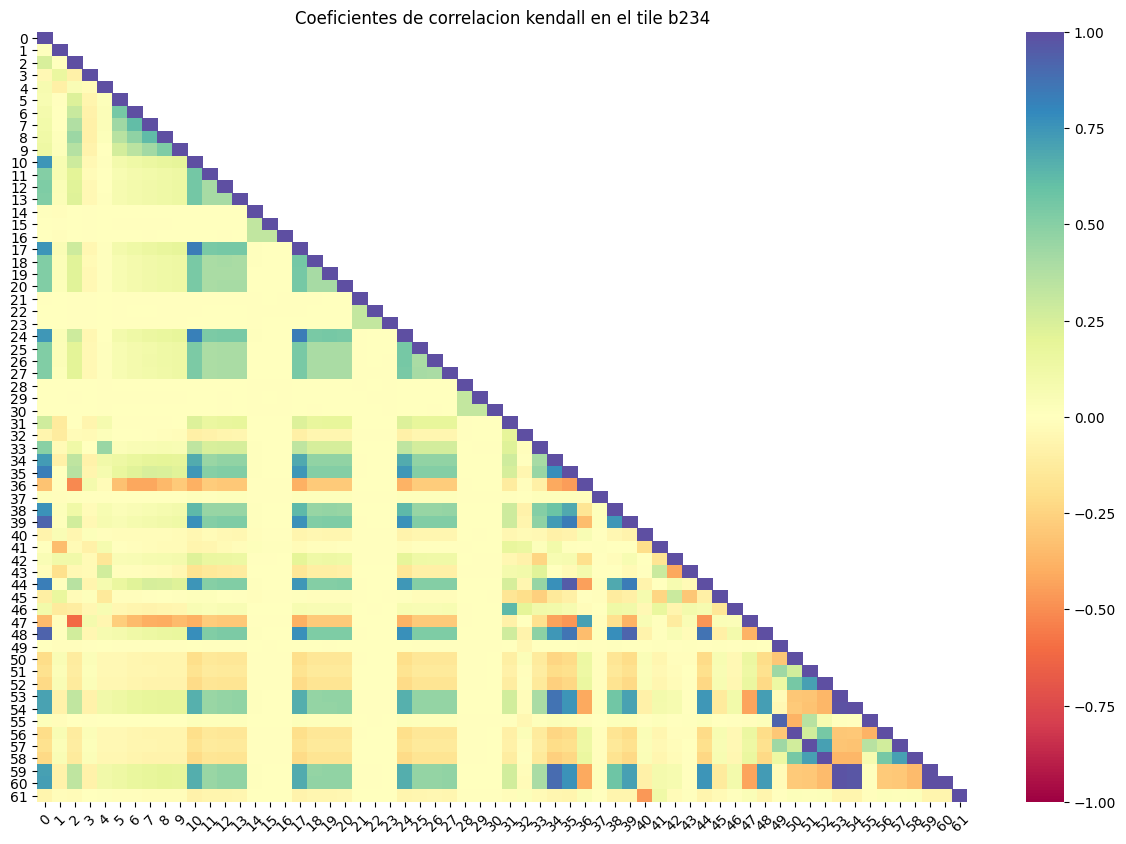
\includegraphics[width=0.49\textwidth]{Kap6/kendall_b234_MATRIX.png}
\end{figure}

\begin{figure}[h!]
\centering
  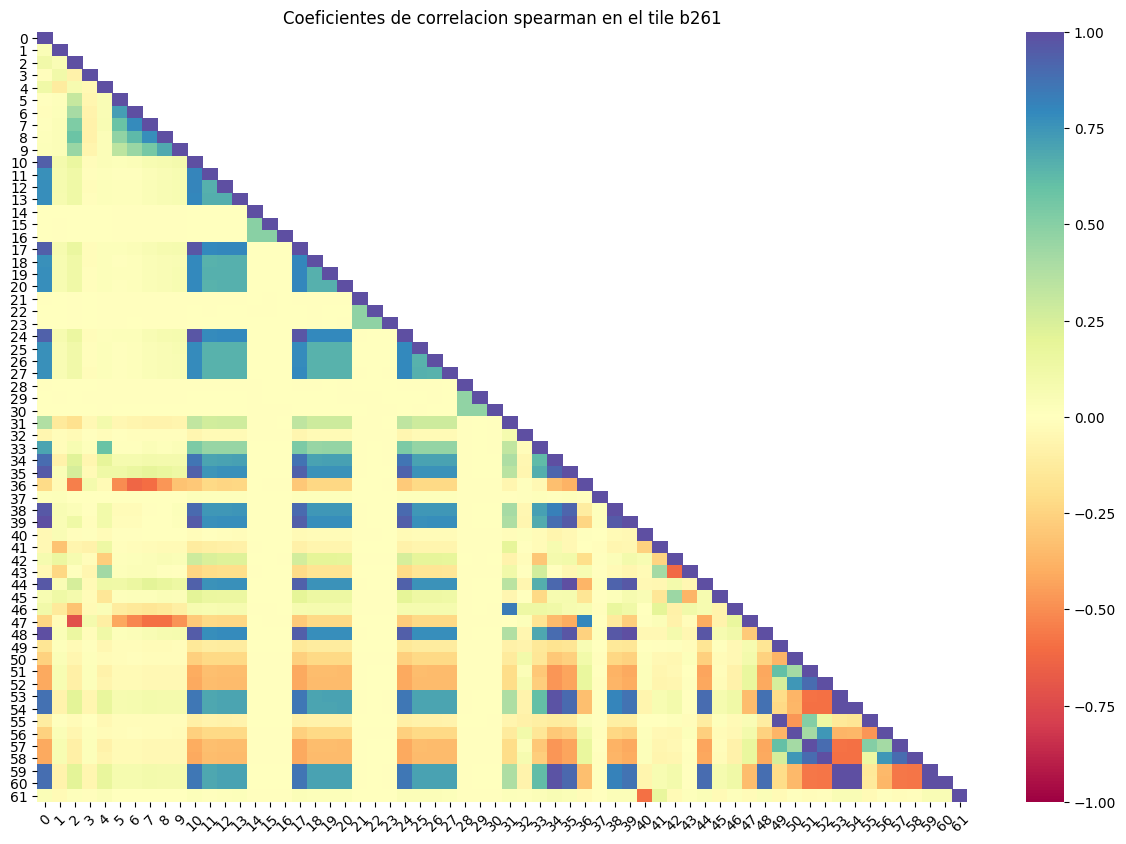
\includegraphics[width=0.49\textwidth]{Kap6/spearman_b261_MATRIX.png} 
  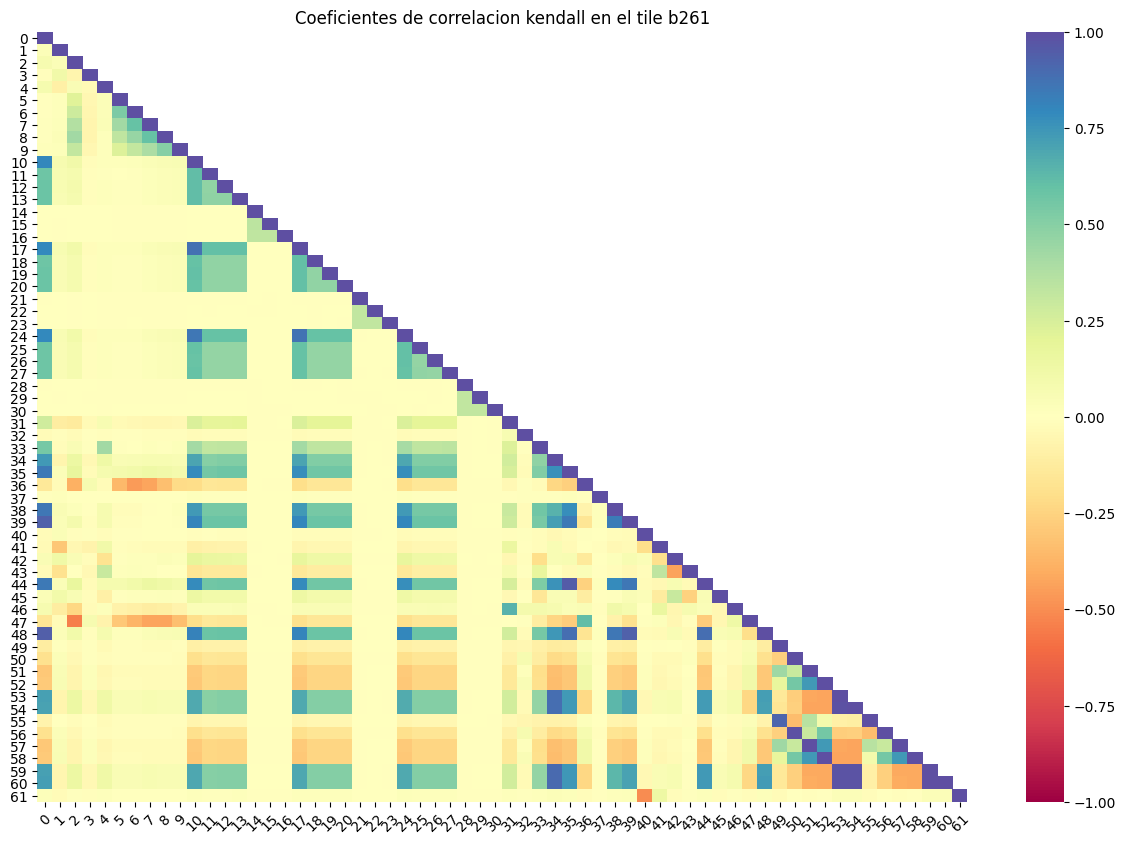
\includegraphics[width=0.49\textwidth]{Kap6/kendall_b261_MATRIX.png} \\
\centering
  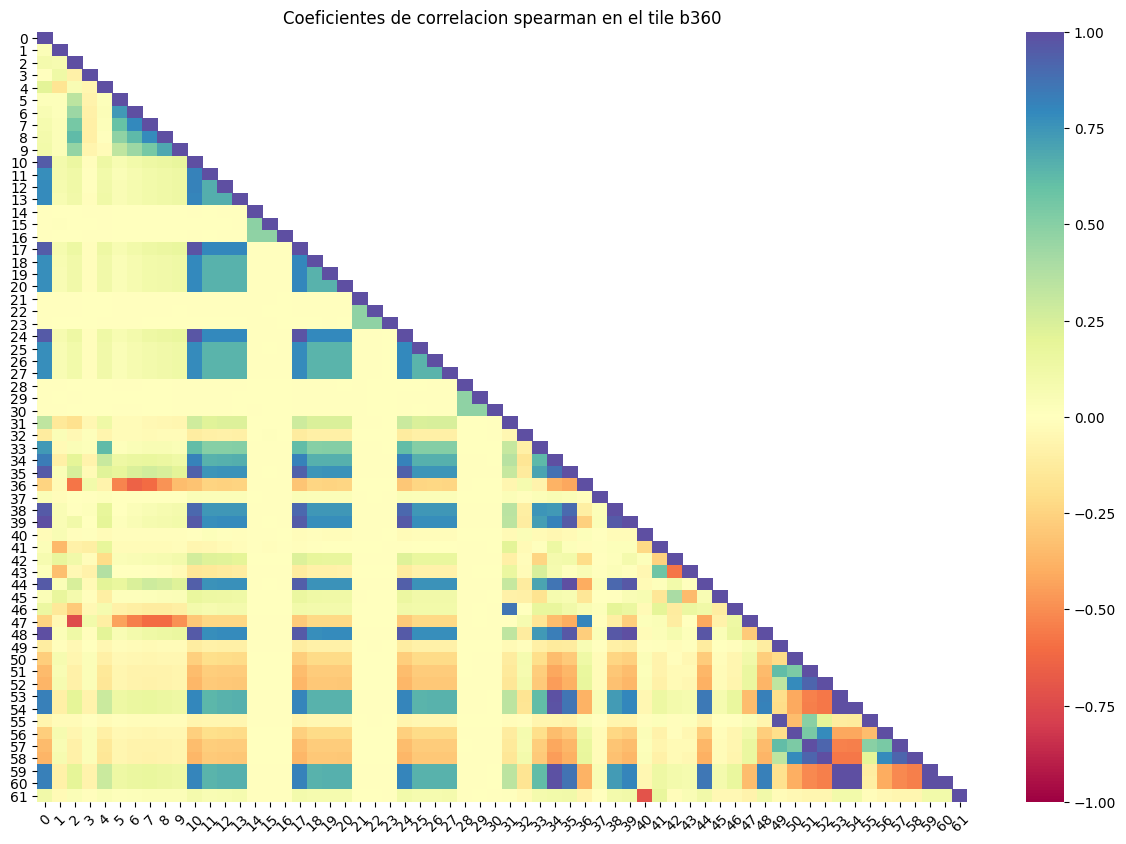
\includegraphics[width=0.49\textwidth]{Kap6/spearman_b360_MATRIX.png} 
  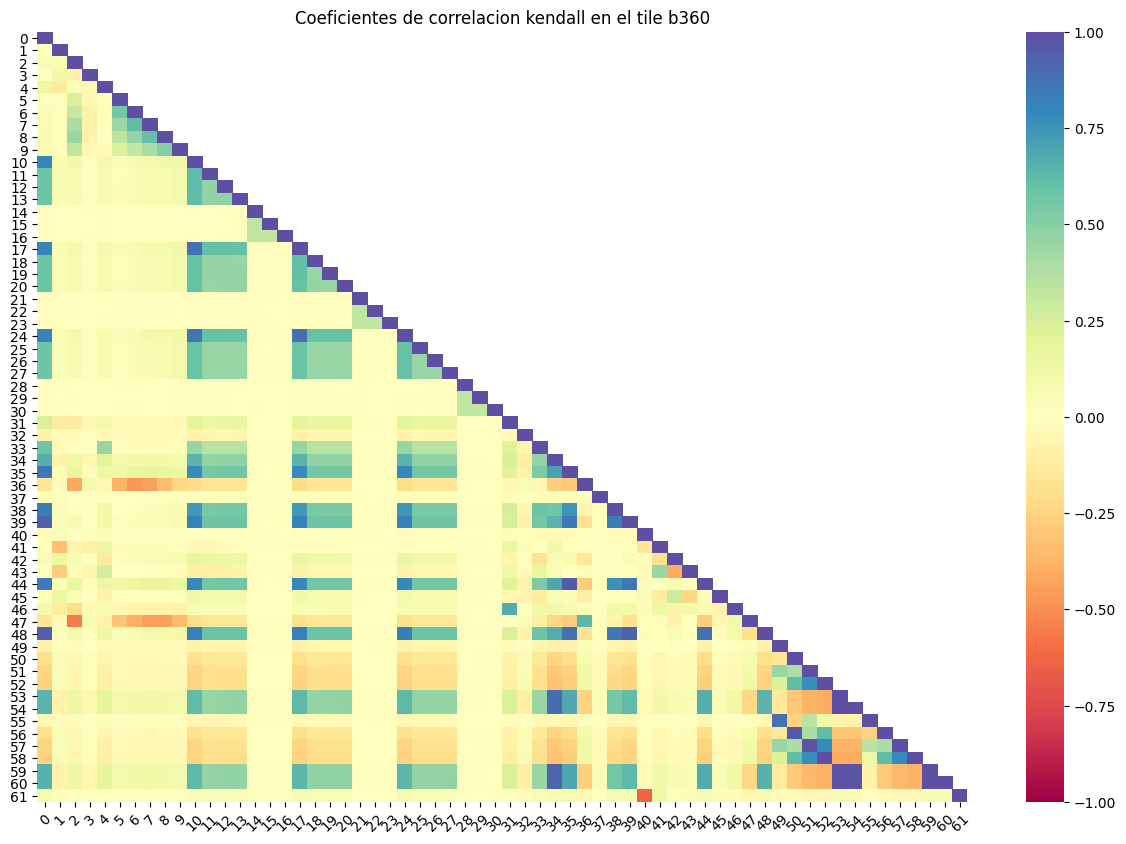
\includegraphics[width=0.49\textwidth]{Kap6/kendall_b360_MATRIX.png}
\end{figure}

\newpage 
\section{Distribuciones de probabilidad de atributos}
\label{anexob_distribuciones}
En esta sección se muestran las distribuciones de probabilidad de los atributos de los tiles b234, b261 y b360.

\begin{figure}[h!]
  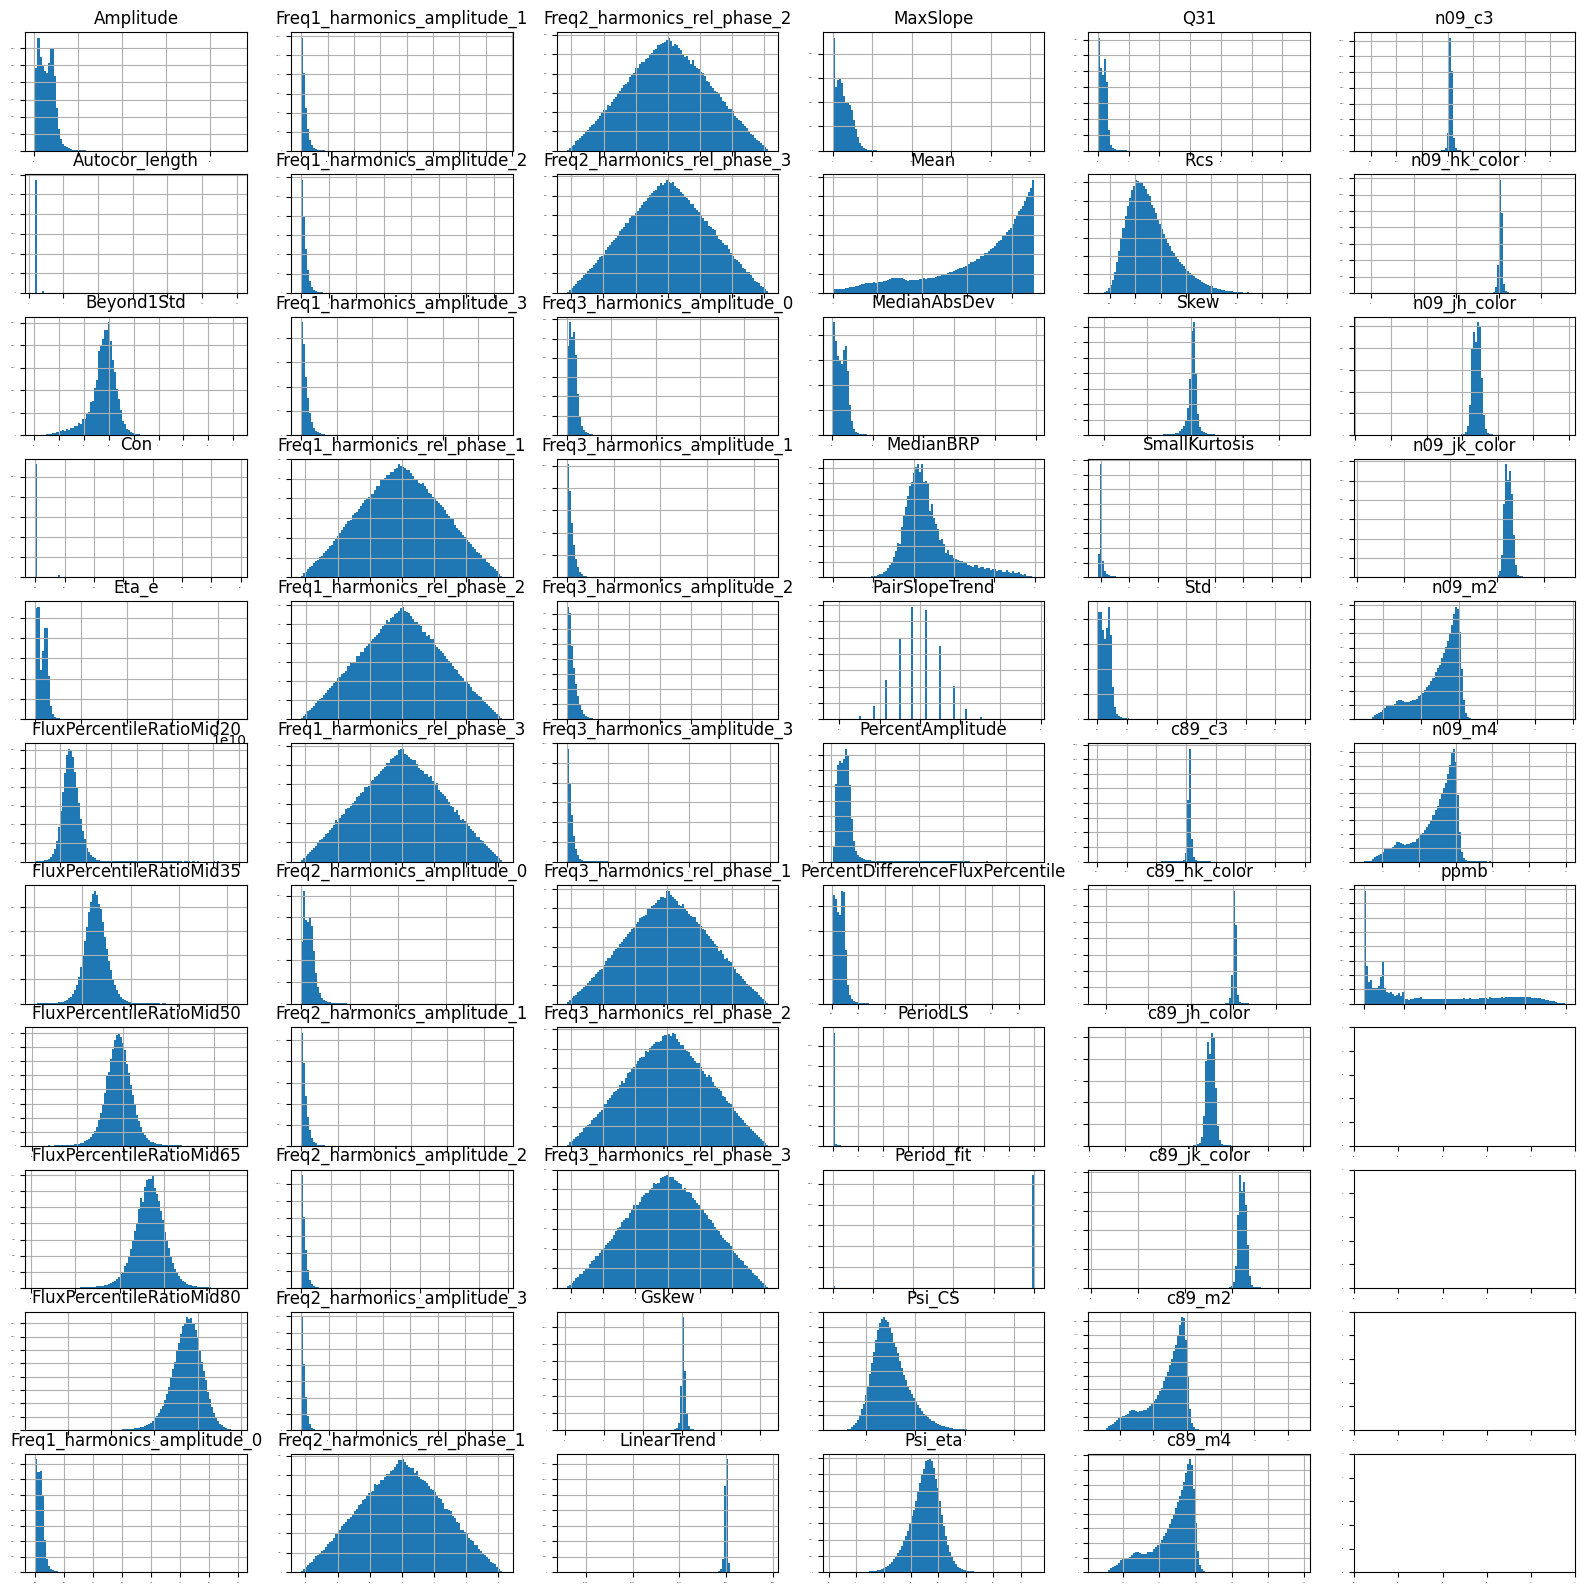
\includegraphics[width=\textwidth]{Kap6/allfeatures_b234.png}
  \caption{Histogramas de frecuencia para los atributos del tile b234}
\end{figure}

\begin{figure}[h!]
  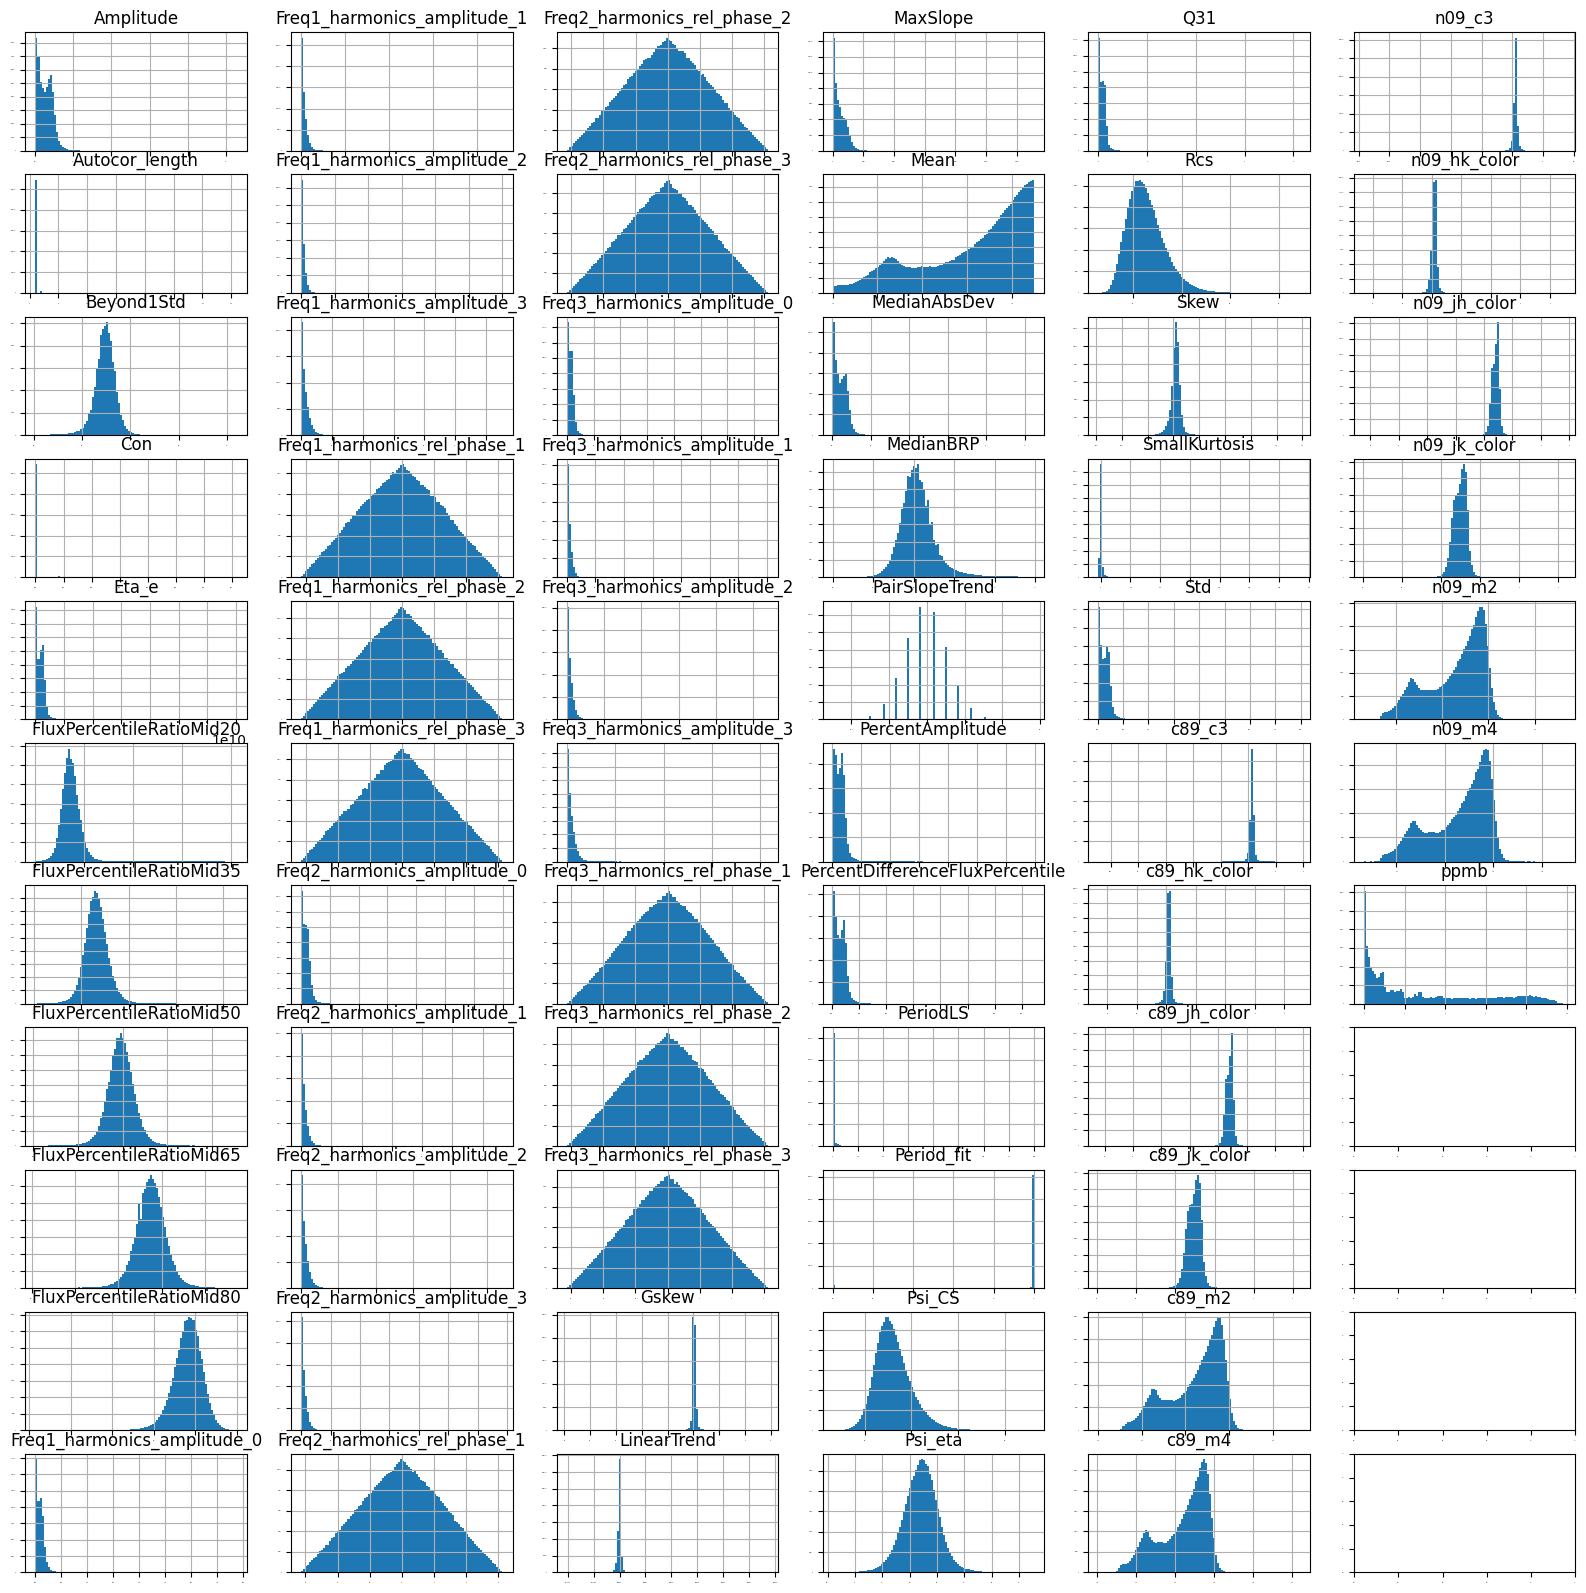
\includegraphics[width=\textwidth]{Kap6/allfeatures_b261.png}
    \caption{Histogramas de frecuencia para los atributos del tile b261}
\end{figure}

\begin{figure}[h!]
  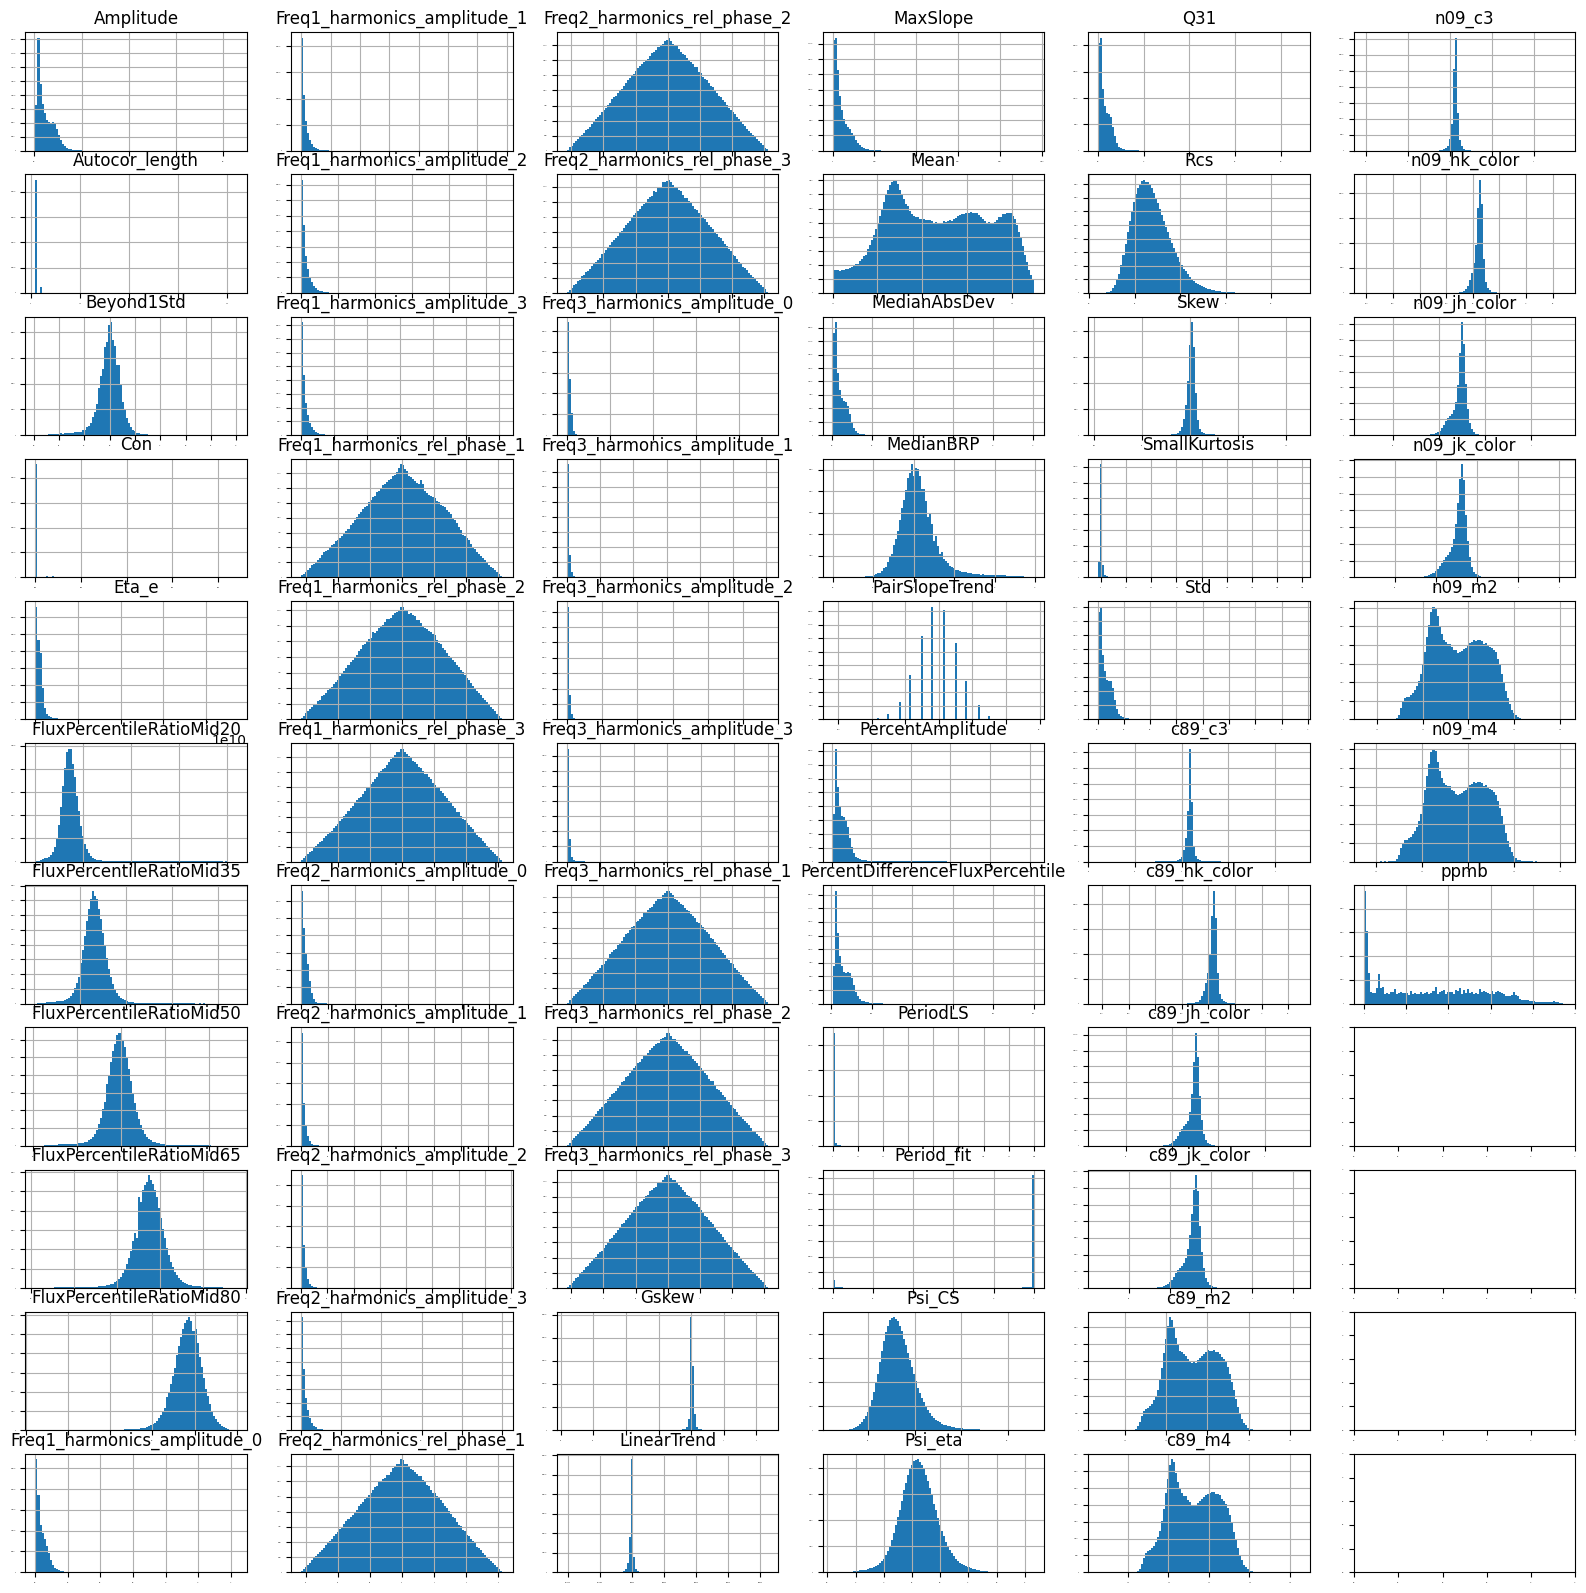
\includegraphics[width=\textwidth]{Kap6/allfeatures_b360.png}
    \caption{Histogramas de frecuencia para los atributos del tile b2360}
\end{figure}

\end{appendix}